\documentclass[12pt]{article}
\usepackage{tikz}
\usepackage{amsmath}
% Underlining package
\usepackage{ulem}
\usetikzlibrary{calc}
\usepackage[a4paper, portrait, margin=1cm]{geometry}
\usepackage{fancyhdr}

\def \HeadingQuestions {\section*{\Large Name: \underline{\hspace{8cm}} \hfill Date: \underline{\hspace{3cm}}} \vspace{-3mm}
{Angles in a Triangle: Questions} \vspace{1pt}\hrule}

% raise footer with page number; no header
\fancypagestyle{myfancypagestyle}{
  \fancyhf{}% clear all header and footer fields
  \renewcommand{\headrulewidth}{0pt} % no rule under header
  \fancyfoot[C] {\thepage} \setlength{\footskip}{6pt} % raise page number 6pt
}
\pagestyle{myfancypagestyle}  % apply myfancypagestyle

\newcounter{minipagecount}

\begin{document}
\HeadingQuestions
\vspace{8mm}

\begin{minipage}{0.55\textwidth}
  \refstepcounter{minipagecount}
  \noindent{(\theminipagecount)}\quad
  \begin{tikzpicture}[scale=1.5, baseline=(current bounding box.north)]
      \pgfmathsetmacro{\angleA}{50}
      \pgfmathsetmacro{\angleB}{54}
      \pgfmathsetmacro{\angleC}{76}
      \pgfmathsetmacro{\sideC}{3.7126720348691356}
      \pgfmathsetmacro{\rotationAngle}{270}
  
    
      \begin{scope}[rotate=\rotationAngle]
        \coordinate (A) at (0,0);
        \coordinate (B) at (\sideC,0);
        \coordinate (C) at (intersection cs: first line={(A)--($(A)+(\angleA:4cm)$)}, second line={(B)--($(B)+(180-\angleB:4cm)$)});
        \draw (A) -- (B) -- (C) -- cycle;
        
        % Mark angles with arcs
        \draw ($(A)!0.3cm!(B)$) arc [start angle=0, end angle=\angleA, radius=0.3cm];
        \draw ($(B)!0.3cm!(C)$) arc [start angle=180-\angleB, end angle=180, radius=0.3cm];
        \draw ($(C)!0.3cm!(A)$) arc [start angle=180+\angleA, end angle=360-\angleB, radius=0.3cm];
        
        % Label angles
        \node at ($(A)!-0.15cm!(B)$) {B};
        \node at ($(B)!-0.15cm!(C)$) {A};
        \node at ($(C)!-0.15cm!(A)$) {C};
        
        % Mark angles in degrees
        \coordinate (midBC) at ($(B)!0.5!(C)$);
        \node at ($(A)!0.55cm!(midBC)$) {$\theta ^\circ$};
    
        \coordinate (midAC) at ($(A)!0.5!(C)$);
        \node at ($(B)!0.55cm!(midAC)$) {54$^\circ$};
    
        \coordinate (midAB) at ($(A)!0.5!(B)$);
        \node at ($(C)!0.55cm!(midAB)$) {76$^\circ$};
      
      \end{scope}
    \end{tikzpicture}
\end{minipage}%
\hfill
\begin{minipage}{0.4\textwidth}
    \begin{align*}
      \angle \text{B} &= 180^\circ - (\angle \text{A} + \angle \text{C}) \\
        &= 180^\circ - (\dotuline{~~~~~~~}^\circ + \dotuline{~~~~~~~}^\circ) \\
        &= 180^\circ - \dotuline{~~~~~~~}^\circ \\
        &= \dotuline{~~~~~~~}^\circ
    \end{align*}
\end{minipage}

\vspace{1cm}\begin{minipage}{0.55\textwidth}
  \refstepcounter{minipagecount}
  \noindent{(\theminipagecount)}\quad
  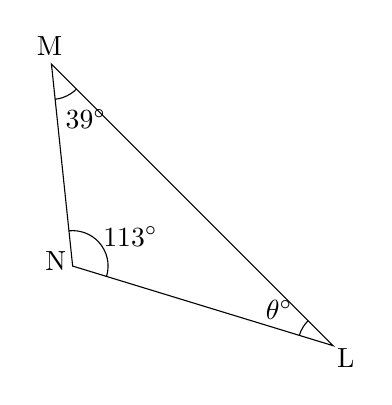
\begin{tikzpicture}[scale=1.5, baseline=(current bounding box.north)]
      \pgfmathsetmacro{\angleA}{28}
      \pgfmathsetmacro{\angleB}{39}
      \pgfmathsetmacro{\angleC}{113}
      \pgfmathsetmacro{\sideC}{3.373333149671335}
      \pgfmathsetmacro{\rotationAngle}{135}
  
    
      \begin{scope}[rotate=\rotationAngle]
        \coordinate (A) at (0,0);
        \coordinate (B) at (\sideC,0);
        \coordinate (C) at (intersection cs: first line={(A)--($(A)+(\angleA:4cm)$)}, second line={(B)--($(B)+(180-\angleB:4cm)$)});
        \draw (A) -- (B) -- (C) -- cycle;
        
        % Mark angles with arcs
        \draw ($(A)!0.3cm!(B)$) arc [start angle=0, end angle=\angleA, radius=0.3cm];
        \draw ($(B)!0.3cm!(C)$) arc [start angle=180-\angleB, end angle=180, radius=0.3cm];
        \draw ($(C)!0.3cm!(A)$) arc [start angle=180+\angleA, end angle=360-\angleB, radius=0.3cm];
        
        % Label angles
        \node at ($(A)!-0.15cm!(B)$) {L};
        \node at ($(B)!-0.15cm!(C)$) {M};
        \node at ($(C)!-0.15cm!(A)$) {N};
        
        % Mark angles in degrees
        \coordinate (midBC) at ($(B)!0.5!(C)$);
        \node at ($(A)!0.55cm!(midBC)$) {$\theta ^\circ$};
    
        \coordinate (midAC) at ($(A)!0.5!(C)$);
        \node at ($(B)!0.55cm!(midAC)$) {39$^\circ$};
    
        \coordinate (midAB) at ($(A)!0.5!(B)$);
        \node at ($(C)!0.55cm!(midAB)$) {113$^\circ$};
      
      \end{scope}
    \end{tikzpicture}
\end{minipage}%
\hfill
\begin{minipage}{0.4\textwidth}
    \begin{align*}
      \angle \text{L} &= 180^\circ - (\angle \text{M} + \angle \text{N}) \\
        &= 180^\circ - (\dotuline{~~~~~~~}^\circ + \dotuline{~~~~~~~}^\circ) \\
        &= 180^\circ - \dotuline{~~~~~~~}^\circ \\
        &= \dotuline{~~~~~~~}^\circ
    \end{align*}
\end{minipage}

\vspace{1cm}\begin{minipage}{0.55\textwidth}
  \refstepcounter{minipagecount}
  \noindent{(\theminipagecount)}\quad
  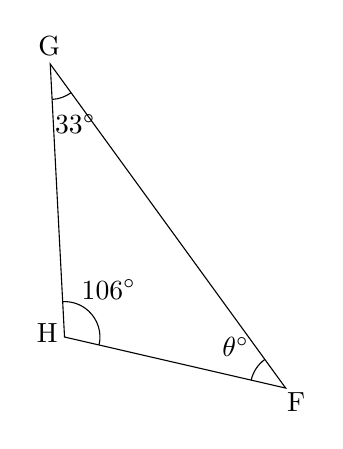
\begin{tikzpicture}[scale=1.5, baseline=(current bounding box.north)]
      \pgfmathsetmacro{\angleA}{41}
      \pgfmathsetmacro{\angleB}{33}
      \pgfmathsetmacro{\angleC}{106}
      \pgfmathsetmacro{\sideC}{3.3908687797631973}
      \pgfmathsetmacro{\rotationAngle}{126}
  
    
      \begin{scope}[rotate=\rotationAngle]
        \coordinate (A) at (0,0);
        \coordinate (B) at (\sideC,0);
        \coordinate (C) at (intersection cs: first line={(A)--($(A)+(\angleA:4cm)$)}, second line={(B)--($(B)+(180-\angleB:4cm)$)});
        \draw (A) -- (B) -- (C) -- cycle;
        
        % Mark angles with arcs
        \draw ($(A)!0.3cm!(B)$) arc [start angle=0, end angle=\angleA, radius=0.3cm];
        \draw ($(B)!0.3cm!(C)$) arc [start angle=180-\angleB, end angle=180, radius=0.3cm];
        \draw ($(C)!0.3cm!(A)$) arc [start angle=180+\angleA, end angle=360-\angleB, radius=0.3cm];
        
        % Label angles
        \node at ($(A)!-0.15cm!(B)$) {F};
        \node at ($(B)!-0.15cm!(C)$) {G};
        \node at ($(C)!-0.15cm!(A)$) {H};
        
        % Mark angles in degrees
        \coordinate (midBC) at ($(B)!0.5!(C)$);
        \node at ($(A)!0.55cm!(midBC)$) {$\theta ^\circ$};
    
        \coordinate (midAC) at ($(A)!0.5!(C)$);
        \node at ($(B)!0.55cm!(midAC)$) {33$^\circ$};
    
        \coordinate (midAB) at ($(A)!0.5!(B)$);
        \node at ($(C)!0.55cm!(midAB)$) {106$^\circ$};
      
      \end{scope}
    \end{tikzpicture}
\end{minipage}%
\hfill
\begin{minipage}{0.4\textwidth}
    \begin{align*}
      \angle \text{F} &= 180^\circ - (\angle \text{G} + \angle \text{H}) \\
        &= 180^\circ - (\dotuline{~~~~~~~}^\circ + \dotuline{~~~~~~~}^\circ) \\
        &= 180^\circ - \dotuline{~~~~~~~}^\circ \\
        &= \dotuline{~~~~~~~}^\circ
    \end{align*}
\end{minipage}

\vspace{1cm}\begin{minipage}{0.55\textwidth}
  \refstepcounter{minipagecount}
  \noindent{(\theminipagecount)}\quad
  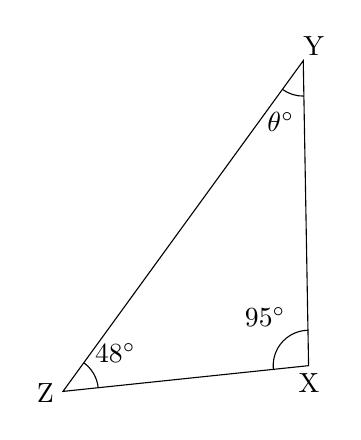
\begin{tikzpicture}[scale=1.5, baseline=(current bounding box.north)]
      \pgfmathsetmacro{\angleA}{37}
      \pgfmathsetmacro{\angleB}{48}
      \pgfmathsetmacro{\angleC}{95}
      \pgfmathsetmacro{\sideC}{3.4608602874931518}
      \pgfmathsetmacro{\rotationAngle}{234}
  
    
      \begin{scope}[rotate=\rotationAngle]
        \coordinate (A) at (0,0);
        \coordinate (B) at (\sideC,0);
        \coordinate (C) at (intersection cs: first line={(A)--($(A)+(\angleA:4cm)$)}, second line={(B)--($(B)+(180-\angleB:4cm)$)});
        \draw (A) -- (B) -- (C) -- cycle;
        
        % Mark angles with arcs
        \draw ($(A)!0.3cm!(B)$) arc [start angle=0, end angle=\angleA, radius=0.3cm];
        \draw ($(B)!0.3cm!(C)$) arc [start angle=180-\angleB, end angle=180, radius=0.3cm];
        \draw ($(C)!0.3cm!(A)$) arc [start angle=180+\angleA, end angle=360-\angleB, radius=0.3cm];
        
        % Label angles
        \node at ($(A)!-0.15cm!(B)$) {Y};
        \node at ($(B)!-0.15cm!(C)$) {Z};
        \node at ($(C)!-0.15cm!(A)$) {X};
        
        % Mark angles in degrees
        \coordinate (midBC) at ($(B)!0.5!(C)$);
        \node at ($(A)!0.55cm!(midBC)$) {$\theta ^\circ$};
    
        \coordinate (midAC) at ($(A)!0.5!(C)$);
        \node at ($(B)!0.55cm!(midAC)$) {48$^\circ$};
    
        \coordinate (midAB) at ($(A)!0.5!(B)$);
        \node at ($(C)!0.55cm!(midAB)$) {95$^\circ$};
      
      \end{scope}
    \end{tikzpicture}
\end{minipage}%
\hfill
\begin{minipage}{0.4\textwidth}
    \begin{align*}
      \angle \text{Y} &= 180^\circ - (\angle \text{Z} + \angle \text{X}) \\
        &= 180^\circ - (\dotuline{~~~~~~~}^\circ + \dotuline{~~~~~~~}^\circ) \\
        &= 180^\circ - \dotuline{~~~~~~~}^\circ \\
        &= \dotuline{~~~~~~~}^\circ
    \end{align*}
\end{minipage}

\vspace{1cm}

\end{document}
